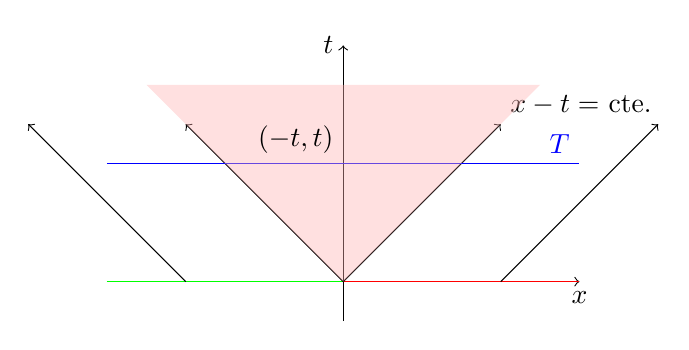
\begin{tikzpicture}

\draw[->] (-3, 0) -- (3,0) node[below] {$x$};
\draw[->] (0, -0.5) -- (0,3) node[left] {$t$};

\draw[green] (-3,0) -- (0,0);
\draw[red] (0,0) -- (3,0);

\draw[->] (0,0) -- (-2,2);
\draw[->] (0,0) -- (2,2) node[above right] {$x-t = $ cte.};
\draw[->] (-2,0) -- (-4,2);
\draw[->] (2,0) -- (4,2);

\draw[blue] (-3,1.5) -- (3,1.5) node[above left] {$T$};

\fill[red!30!white, opacity = 0.4] (0,0) -- (-2.5,2.5) -- (2.5,2.5) -- cycle;

\draw (0,1.5) node[above left] {$(-t,t)$};

\end{tikzpicture}